% Created 2020-07-24 vie 12:26
% Intended LaTeX compiler: pdflatex
\documentclass[presentation,aspectratio=1610]{beamer}
\usepackage[utf8]{inputenc}
\usepackage[T1]{fontenc}
\usepackage{graphicx}
\usepackage{grffile}
\usepackage{longtable}
\usepackage{wrapfig}
\usepackage{rotating}
\usepackage[normalem]{ulem}
\usepackage{amsmath}
\usepackage{textcomp}
\usepackage{amssymb}
\usepackage{capt-of}
\usepackage{hyperref}
\usepackage{pifont}
\newcommand{\cmark}{\textcolor{green!80!black}{\ding{51}}}
\usepackage{amssymb}
\usepackage{pgfplotstable}
\DeclareMathOperator{\shift}{q}
\DeclareMathOperator{\diff}{p}
\usepackage{khpreamble, euscript}
\DeclareMathOperator{\atantwo}{atan2}
\newcommand*{\ctrb}{\EuScript{C}}
\newcommand*{\obsv}{\EuScript{O}}
\usetheme{default}
\author{Kjartan Halvorsen}
\date{\today}
\title{Control computarizado - Modelos en espacio de estado}
\hypersetup{
 pdfauthor={Kjartan Halvorsen},
 pdftitle={Control computarizado - Modelos en espacio de estado},
 pdfkeywords={},
 pdfsubject={},
 pdfcreator={Emacs 26.3 (Org mode 9.3.6)}, 
 pdflang={English}}
\begin{document}

\maketitle

\section{PMSM - Motor syncrono de Iman permanente, sysid}
\label{sec:org75c5f79}


\begin{frame}[label={sec:org504525b}]{PMSM - Motor síncrono de imán permanente}
\begin{center}
\includegraphics[width=0.9\linewidth]{../../figures/permanent-motor.jpg}
\end{center}
\end{frame}

\begin{frame}[label={sec:orgc3bdbca}]{PMSM - Motor síncrono de imán permanente}
\begin{center}
\includegraphics[width=0.8\linewidth]{../../figures/pmsm_control_block_diag.png}
\end{center}
{\footnotesize De Liu and Li  ``Speed control for PMSM servo system'', IEEE Transactions on Industrial Electronics, 2012.}
\end{frame}
\begin{frame}[label={sec:orgd3657b8}]{Modelo identificado}
Dos polos, dos ceros, un retraso
\begin{center}
  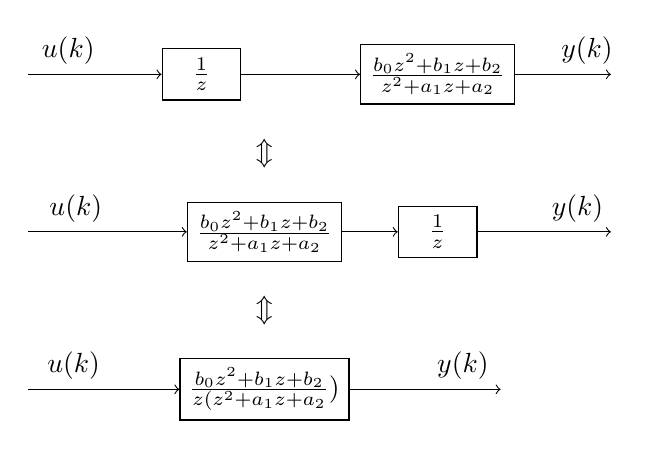
\begin{tikzpicture}[node distance=22mm, block/.style={rectangle, draw, minimum width=10mm}, sumnode/.style={circle, draw, inner sep=2pt}]

    \node[coordinate] (input) {};
    \node[block, right of=input] (delay1)  {$\frac{1}{z}$};
    \node[block, right of=delay1, node distance=30mm] (plant)  {$\frac{b_0z^2 + b_1z + b_2}{z^2 + a_1 z + a_2}$};
    \node[coordinate, right of=plant] (output) {};

    \draw[->] (input) -- node[above, pos=0.3] {$u(k)$} (delay1);
    \draw[->] (delay1) -- node[above, pos=0.3] {} (plant);
    \draw[->] (plant) -- node[above, near end] {$y(k)$} (output);

    \begin{scope}[yshift=-1cm, xshift = 3cm]
    \node {$\Updownarrow$};
    \end{scope}
    \begin{scope}[yshift=-3cm, xshift = 3cm]
    \node {$\Updownarrow$};
    \end{scope}

    \node[coordinate, below of=input, node distance=2cm] (input2) {};
    \node[block, right of=input2, node distance=30mm] (plant)  {$\frac{b_0z^2 + b_1z + b_2}{z^2 + a_1 z + a_2}$};
    \node[block, right of=plant] (delay2)  {$\frac{1}{z}$};
    \node[coordinate, right of=delay2] (output) {};

    \draw[->] (input2) -- node[above, pos=0.3] {$u(k)$} (plant);
    \draw[->] (plant) -- node[above, pos=0.3] {} (delay2);
    \draw[->] (delay2) -- node[above, near end] {$y(k)$} (output);

    \node[coordinate, below of=input2, node distance=2cm] (input3) {};
    \node[block, right of=input3, node distance=30mm] (plant)  {$\frac{b_0z^2 + b_1z + b_2}{z(z^2 + a_1 z + a_2})$};
    \node[coordinate, right of=plant, node distance=30mm] (output) {};

    \draw[->] (input3) -- node[above, pos=0.3] {$u(k)$} (plant);
    \draw[->] (plant) -- node[above, near end] {$y(k)$} (output);



  \end{tikzpicture}
\end{center}
\end{frame}

\begin{frame}[label={sec:org823e0e7}]{Model ARX}
Dado señales \(u(k), \; k=1,2,\ldots, N\) y \(y(k), \; k=1,2,\ldots,N\), el modelo ARX \(A(\shift)y(k) = B(\shift)u(k-d) + \shift^n e(k)\) con \(n\) polos, \(m\) ceros y retraso de \(d\) pasos.

\alert{Predictor}
\begin{multline*}
\hat{y}(k+1) = -a_1y(k) - \cdots - a_ny(k-n+1) \\+ b_0u(k+m-n-d+1) + \cdots + b_mu(k-n-d+1)
\end{multline*}
\alert{Objetivo} Estimar los parametro \(a_1, a_2, \ldots, \a_n, b_0, b_1, \ldots, b_m\).

\alert{Modelo del PMSM} \(n=2\), \(m=2\), \(d=1\)
\begin{multline*}
\hat{y}(k+1) = -a_1y(k) - a_2y(k-1) + b_0u(k) + b_1u(k-1) + b_2u(k-2)d+1) 
\end{multline*}
\end{frame}

\begin{frame}[label={sec:org40544ae}]{Modelo identificado}
\[ H(z) = \frac{6.91z^2 + 16.48z -17.87}{z(z^2 - 1.766z + 0.7665)} = \frac{6.91(z+3.19)(z-0.81)}{z(z-0.998)(z-0.768)}\]

\begin{center}
\includegraphics[width=0.6\linewidth]{../../figures/validation-result-2020-07-24.png}
\end{center}
\end{frame}

\begin{frame}[label={sec:org5cf3932}]{De función de transferencia a modelo en espacio  de estados}
\begin{center}
  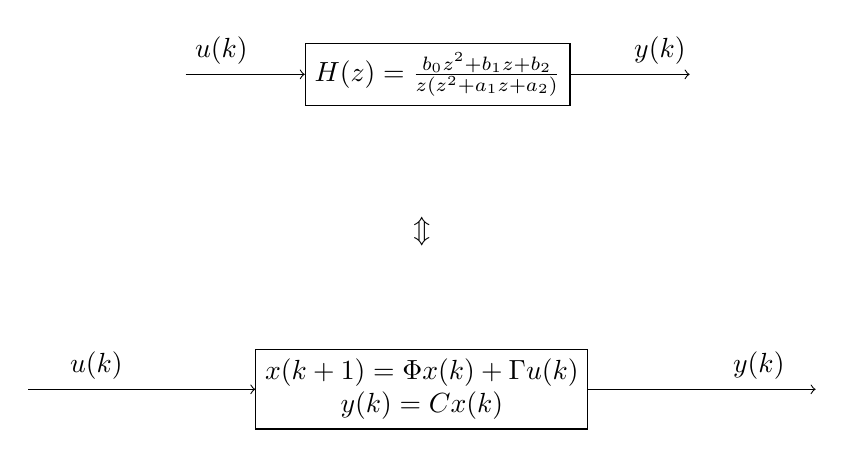
\begin{tikzpicture}[node distance=32mm, block/.style={rectangle, draw, minimum width=15mm}, sumnode/.style={circle, draw, inner sep=2pt}]

    \node[coordinate] (input) {};
    \node[block, right of=input] (plant)  {$H(z) = \frac{b_0z^2 + b_1z + b_2}{z(z^2 + a_1 z + a_2)}$};
    \node[coordinate, right of=plant] (output) {};

    \draw[->] (input) -- node[above, pos=0.3] {$u(k)$} (plant);
    \draw[->] (plant) -- node[above, near end] {$y(k)$} (output);

    \begin{scope}[yshift=-2cm, xshift = 3cm]
    \node {$\Updownarrow$};
    \end{scope}

    \begin{scope}[yshift=-4cm, node distance=50mm, xshift=-2cm]
    \node[coordinate] (input) {};
    \node[block, right of=input, align=center] (plant)  {$x(k+1) = \Phi x(k) + \Gamma u(k)$\\$y(k) = C x(k)$};
    \node[coordinate, right of=plant] (output) {};

    \draw[->] (input) -- node[above, pos=0.3] {$u(k)$} (plant);
    \draw[->] (plant) -- node[above, near end] {$y(k)$} (output);
    \end{scope}



  \end{tikzpicture}
\end{center}
\end{frame}

\begin{frame}[label={sec:orga29fe05}]{Formas canónicas}
Dado función de transferencia 
\[ H(z) = \frac{b_1 z^2 + b_2 z + b_3}{z^3 + a_1z^2 + a_2z + a_3}.\] 
Encuentra una representación en espacio de estado.
\begin{align*}
 x(k+1) &= \Phi x(k) + \Gamma u(k) \\
 y(k) &= C x(k)
 \end{align*}

\begin{itemize}
\item Forma canónica de control
\item Forma canónica de observador
\end{itemize}
\end{frame}

\begin{frame}[label={sec:orgb2760c7}]{Forma canónica de control}
Dado función de transferencia 
\[ H(z) = \frac{b_1 z^2 + b_2 z + b_3}{z^3 + a_1z^2 + a_2z + a_3}.\] 

\begin{align*}
 x(k+1) &= \begin{bmatrix} -a_1 & -a_2 & -a_3\\1 & 0 & 0\\0 & 1 & 0\end{bmatrix} x(k) + \begin{bmatrix}1\\0\\0\end{bmatrix} u(k) \\
 y(k) &= \begin{bmatrix} b_1 & b_2 & b_3 \end{bmatrix} x(k)
 \end{align*}
\end{frame}


\begin{frame}[label={sec:org86f0584}]{Forma canónica de observador}
Dado función de transferencia 
\[ H(z) = \frac{b_1 z^2 + b_2 z + b_3}{z^3 + a_1z^2 + a_2z + a_3}.\] 

\begin{align*}
 x(k+1) &= \begin{bmatrix} -a_1 & 1 & 0\\-a_2 & 0 & 1\\-a_3 & 0 & 0\end{bmatrix} x(k) + \begin{bmatrix}b_1\\b_2\\b_3\end{bmatrix} u(k) \\
 y(k) &= \begin{bmatrix} 1 & 0 & 0 \end{bmatrix} x(k)
 \end{align*}
\end{frame}


\begin{frame}[label={sec:org72d914f}]{Formas canónicas - ejercicio}
\alert{Actividad} Encuentra las formas canónicas de control y de observador para la función de transferencia del motor
\[ H(z) = \frac{6.91z^2 + 16.48z -17.87}{z(z^2 - 1.766z + 0.7665)} = \frac{6.91(z+3.19)(z-0.81)}{z(z-0.998)(z-0.768)}\]
\end{frame}

\begin{frame}[label={sec:org8e71ee4}]{Formas canónicas - solución}
\end{frame}
\begin{frame}[label={sec:orgec43f7d}]{Formas canónicas - solución}
\[ H(z) = \frac{6.91z^2 + 16.48z -17.87}{z(z^2 - 1.766z + 0.7665)} = \frac{6.91(z+3.19)(z-0.81)}{z(z-0.998)(z-0.768)}\]
Forma canónica de control
\begin{align*}
 x(k+1) &= \begin{bmatrix} -a_1 & -a_2 & -a_3\\1 & 0 & 0\\0 & 1 & 0\end{bmatrix} x(k) + \begin{bmatrix}1\\0\\0\end{bmatrix} u(k) \\
   &= \begin{bmatrix} 1.766 & -0.7655 & 0\\1 & 0 & 0\\0 &1 & 0\end{bmatrix} x(k) +  \begin{bmatrix}1\\0\\0\end{bmatrix} u(k) \\
 y(k) &= \begin{bmatrix} b_1 & b_2 & b_3 \end{bmatrix} x(k)
 = \begin{bmatrix} 6.91 & 16.48 & -17.87 \end{bmatrix} x(k)
 \end{align*}
\end{frame}


\begin{frame}[label={sec:org971ea4a}]{Formas canónicas - solución}
\[ H(z) = \frac{6.91z^2 + 16.48z -17.87}{z(z^2 - 1.766z + 0.7665)} = \frac{6.91(z+3.19)(z-0.81)}{z(z-0.998)(z-0.768)}\]
Forma canónica de observador
\begin{align*}
 x(k+1) &= \begin{bmatrix} -a_1 & 1 & 0\\-a_2 & 0 & 1\\-a_3 & 0 & 0\end{bmatrix} x(k) + \begin{bmatrix}b_1\\b_2\\b_3\end{bmatrix} u(k) \\
 &= \begin{bmatrix} 1.766 & 1 & 0\\-0.7665 & 0 & 1\\0 & 0 & 0\end{bmatrix} x(k) + \begin{bmatrix}6.91\\16.48\\-17.87\end{bmatrix} u(k) \\
 y(k) &= \begin{bmatrix} 1 & 0 & 0 \end{bmatrix} x(k)
 \end{align*}
\end{frame}

\section{Apollo moon lander}
\label{sec:org516015a}
\begin{frame}[label={sec:orgd2f009f}]{Modelación en espacio de estado}
\end{frame}
\begin{frame}[label={sec:org734459f}]{Ejemplo - El módulo lunar de Apollo}
\begin{center}
\includegraphics[width=\linewidth]{fig-apollo}
\end{center}
\end{frame}
\begin{frame}[label={sec:org74bf6ca}]{Ejemplo - El módulo lunar de Apollo}
\begin{center}
\includegraphics[width=0.8\linewidth]{fig-apollo}
\end{center}
\alert{Actividad} ¿Cuál es la función de transferencia del sistema?
\[1: \; G(s) = \frac{k_1 k_2}{s^2}\qquad 2: \; G(s) = \frac{k_1 k_2}{s(s^2 + 1)} \qquad 3: \; G(s) = \frac{k_1 k_2}{s^3}\]
\end{frame}

\begin{frame}[label={sec:orgd78927d}]{Ejemplo - El módulo lunar de Apollo}
\begin{center}
\includegraphics[width=0.8\linewidth]{fig-apollo}
\end{center}
\alert{Actividad} ¿Que sensores relevantes se puede usar para el control?
\end{frame}

\begin{frame}[label={sec:orgcb1614f}]{Ejemplo - El módulo lunar de Apollo}
\begin{center}
\includegraphics[width=0.7\linewidth]{fig-apollo}
\end{center}

Variables del estado: \(x = \begin{bmatrix} x_1 & x_2 & x_3 \end{bmatrix}^T = \begin{bmatrix} \dot{\theta} & \theta & \dot{z} \end{bmatrix}^T\). Con dinamica
\[ \begin{cases} \dot{x}_1 =  \ddot{\theta} = k_1 u\\ \dot{x}_2 = \dot{\theta} = x_1\\ \dot{x}_3 = \ddot{z} = k_2\theta = k_2x_2 \end{cases} \]
\end{frame}

\begin{frame}[label={sec:orgd55f7a8}]{Ejemplo - El módulo lunar de Apollo}
Variables del estado: \(x = \begin{bmatrix} x_1 & x_2 & x_3 \end{bmatrix}^T = \begin{bmatrix} \dot{\theta} & \theta & \dot{z} \end{bmatrix}^T\). Con dinamica
\[ \begin{cases} \dot{x}_1 =  \ddot{\theta} = k_1 u\\ \dot{x}_2 = \dot{\theta} = x_1\\ \dot{x}_3 = \ddot{z} = k_2\theta = k_2x_2 \end{cases} \]

\alert{Actividad} Llena las matriz \(A\) y vector \(B\) en el modelo de espacio de estado

\[ \dot{x} = \begin{bmatrix} \dot{x}_1\\\dot{x}_2\\\dot{x}_3\end{bmatrix} = \underbrace{\begin{bmatrix} \textcolor{white}{0} & \textcolor{white}{0} &\textcolor{white}{0} \\\textcolor{white}{1} & \textcolor{white}{0}& \textcolor{white}{0}\\ \textcolor{white}{0}& \textcolor{white}{k_2} &\textcolor{white}{0} \end{bmatrix}}_{A} \begin{bmatrix} x_1\\x_2\\x_3\end{bmatrix} + \underbrace{\begin{bmatrix} \textcolor{white}{k_1} \\ \textcolor{white}{0} \\\textcolor{white}{0}  \end{bmatrix}}_{B} u \]
\end{frame}

\begin{frame}[label={sec:org79e4302}]{Ejemplo - El módulo lunar de Apollo - Solución}
\end{frame}

\begin{frame}[label={sec:orgd079e52}]{Ejemplo - El módulo lunar de Apollo - Solución}
Variables del estado: \(x = \begin{bmatrix} x_1 & x_2 & x_3 \end{bmatrix}^T = \begin{bmatrix} \dot{\theta} & \theta & \dot{z} \end{bmatrix}^T\). Con dinamica
\[ \begin{cases} \dot{x}_1 =  \ddot{\theta} = k_1 u\\ \dot{x}_2 = \dot{\theta} = x_1\\ \dot{x}_3 = \ddot{z} = k_2\theta = k_2x_2 \end{cases} \]

\alert{Actividad} Llena las matriz \(A\) y vector \(B\) en el modelo de espacio de estado

\[ \dot{x} = \begin{bmatrix} \dot{x}_1\\\dot{x}_2\\\dot{x}_3\end{bmatrix} = \underbrace{\begin{bmatrix} \textcolor{red!60!black}{0} & \textcolor{red!60!black}{0} &\textcolor{red!60!black}{0} \\\textcolor{red!60!black}{1} & \textcolor{red!60!black}{0}& \textcolor{red!60!black}{0}\\ \textcolor{red!60!black}{0}& \textcolor{red!60!black}{k_2} &\textcolor{red!60!black}{0} \end{bmatrix}}_{A} \begin{bmatrix} x_1\\x_2\\x_3\end{bmatrix} + \underbrace{\begin{bmatrix} \textcolor{red!60!black}{k_1} \\ \textcolor{red!60!black}{0} \\\textcolor{red!60!black}{0}  \end{bmatrix}}_{B} u \]
\end{frame}


\begin{frame}[label={sec:org83e8e02}]{Modelación - ejercicio}
\alert{Actividad} Las siguientes diapositivas enseñan tres ejemplos de modelos en espacio de estado. A cada breakout room se asigna un modelo

\begin{center}
\begin{tabular}{llllrrrrrr}
Modelo $\backslash$ Breakout room & 1 & 2 & 3 & 4 & 5 & 6 & 7 & 8 & 9\\
\hline
A & \cmark & \cmark & \cmark &  &  &  &  &  & \\
B &  &  &  & \cmark & \cmark & \cmark &  &  & \\
C &  &  &  &  &  &  & \cmark & \cmark & \cmark\\
\hline
\end{tabular}
\end{center}

\alert{Interpreta el modelo} ¿Cuales son los variables de estado, que significan y que unidad tienen? ¿Cuál es la señal de entrada y la señal de salida? ¿Qué unidad tienen esas señales? ¿De dónde  viene el modelo (leyes físicas, ecuaciones diferenciales)?

\alert{Prepara un breve explicación} con ayuda a los recursos dados.
\end{frame}

\begin{frame}[label={sec:org587b783}]{Modelación - Modelo \alert{A}}
\begin{columns}
\begin{column}{0.5\columnwidth}
\includegraphics[height=0.5\textheight]{../../figures/mass-spring-damper}
\end{column}

\begin{column}{0.5\columnwidth}
Movimiento vertical de una masa. En la posición relajada, \(X=0, \; \dot{X} =0\), la fuerza en el resorte es igual a la fuerza de gravedad.  

\begin{align*}
\dot{x} &= \begin{bmatrix} 0 & 1\\-\frac{k}{m} & -\frac{f}{m}\end{bmatrix} x + \begin{bmatrix}0\\\frac{k}{m}\end{bmatrix}u\\ 
y &= \begin{bmatrix} 1 & 0\end{bmatrix} x 
\end{align*}

\href{https://lpsa.swarthmore.edu/Representations/SysRepSS.html\#SS\_MechT}{Liga a recurso}
\end{column}
\end{columns}
\end{frame}

\begin{frame}[label={sec:orgbe8658e}]{Modelación - Modelo \alert{B}}
\begin{columns}
\begin{column}{0.5\columnwidth}
\includegraphics[height=0.5\textheight]{../../figures/RLC-circuit}
\end{column}


\begin{column}{0.5\columnwidth}
Tip: \(x_1(t) = i(t)\)

\begin{align*}
\dot{x} &= \begin{bmatrix} -\frac{R}{L} & -\frac{1}{L}\\\frac{1}{C} & 0\end{bmatrix} x + \begin{bmatrix}\frac{1}{L}\\0\end{bmatrix}u\\ 
y &= \begin{bmatrix} 0 & 1\end{bmatrix} x 
\end{align*}

\href{https://lpsa.swarthmore.edu/Representations/SysRepSS.html\#ExDirDerSSElec}{Liga a recurso}
\end{column}
\end{columns}
\end{frame}


\begin{frame}[label={sec:orgff1ee19}]{Modelación - Modelo \alert{C}}
\begin{columns}
\begin{column}{0.5\columnwidth}
\includegraphics[height=0.5\textheight]{../../figures/two-tank-mathworks.png}

{\footnotesize From Mathworks}
\end{column}

\begin{column}{0.5\columnwidth}
\begin{align*}
\dot{x} &= \begin{bmatrix} -\frac{a}{A} \sqrt{2gx_1}\\ \frac{a}{A}\sqrt{2gx_1} - \frac{a}{A}\sqrt{2gx_2}\end{bmatrix} + \begin{bmatrix}\frac{k}{A}\\0\end{bmatrix}u\\ 
y &= \begin{bmatrix} 0 & 1\end{bmatrix} x 
\end{align*}

\href{https://www.mathworks.com/help/ident/examples/two-tank-system-c-mex-file-modeling-of-time-continuous-siso-system.html}{Liga a recurso}
\end{column}
\end{columns}
\end{frame}

\section{Discretización}
\label{sec:org26f2aef}

\begin{frame}[label={sec:org70b86e0}]{Discretización}
\end{frame}
\begin{frame}[label={sec:org03e5974}]{Discretización}
Solución general de un sistema lineal en espacio de estado 
\begin{align*}
x(t_k+\tau)& = \mathrm{e}^{A(\tau)} x(t_k) + \int_{0}^\tau \mathrm{e}^{As} B u\big((t_k+\tau)-s) ds
\end{align*}

\begin{center}
  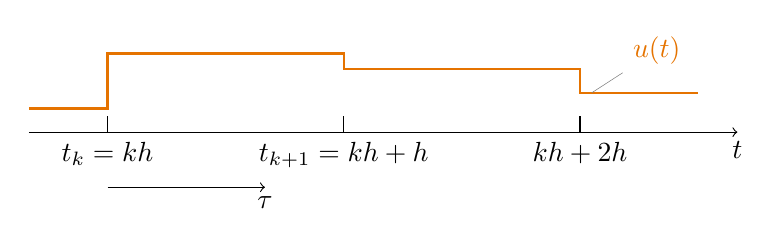
\begin{tikzpicture}
    \draw[->] (-3,0) -- (6,0) node[below] {$t$};
    \draw (-2, 0.2) -- ( -2, 0) node[below] {$t_k=kh$};
    \draw (1, 0.2) -- ( 1, 0) node[below] {$t_{k+1}=kh+h$};
    \draw (4, 0.2) -- ( 4, 0) node[below] {$kh+2h$};
    \draw[thick, orange!90!black] (-3,0.3) -- (-2, 0.3) -- (-2,1) -- (1, 1) -- (1,0.8) -- (4, 0.8) --(4, 0.5) --(5.5, 0.5) node[pos=0.1, coordinate, pin=30:{$u(t)$}] {} ; 
    \draw[->] (-2, -0.7) -- (0, -0.7) node[below] {$\tau$};
  \end{tikzpicture}
\end{center}

 \begin{align*}
  x(kh+h) &= \mathrm{e}^{Ah} x(kh) + \int_{0}^{h} \mathrm{e}^{As} B u(kh+h-s) ds\\
   &= \underbrace{\mathrm{e}^{Ah}}_{\Phi(h)} x(kh) + \underbrace{\left(\int_{0}^h \mathrm{e}^{As} B ds \right)}_{\Gamma(h)} u(kh)
\end{align*}
\end{frame}

\begin{frame}[label={sec:orge27338d}]{Discretización - La exponencial de una matriz}
Matriz \(A\) cuadrada. Variable \(t\) escalar.
\[ \mathrm{e}^{At} = 1 + At + \frac{t^2}{2!}A^2 + \frac{t^3}{3!} A^3 + \cdots\]
Transformada de Laplace:
\[ \laplace{\mathrm{e}^{At}} = (sI - A)^{-1}\]
\end{frame}


\begin{frame}[label={sec:org3cae162}]{Discretización - ejemplo}
 \begin{align*}
  x(kh+h) &= \mathrm{e}^{Ah} x(kh) + \int_{0}^{h} \mathrm{e}^{As} B u(kh+h-s) ds\\
   &= \underbrace{\mathrm{e}^{Ah}}_{\Phi(h)} x(kh) + \underbrace{\left(\int_{0}^h \mathrm{e}^{As} B ds \right)}_{\Gamma(h)} u(kh)
\end{align*}
\[ A = \begin{bmatrix} 0 & 0 & 0\\1 & 0 & 0\\0 & k_2 & 0\end{bmatrix}, \quad A^2 = \begin{bmatrix} 0 & 0 & 0\\1 & 0 & 0\\0 & k_2 & 0\end{bmatrix}\begin{bmatrix} 0 & 0 & 0\\1 & 0 & 0\\0 & k_2 & 0\end{bmatrix}= \begin{bmatrix} 0 & 0 & 0\\0 & 0 & 0\\k_2 & 0  & 0\end{bmatrix}, \quad A^3 = 0\]
Entonces,
\begin{align*}
 \Phi(h) &= \mathrm{e}^{Ah} = 1 + Ah + A^2 h^2/2  + \cdots \\
 &= \begin{bmatrix} 1 & 0 & 0\\0 & 1 & 0\\0 & 0 & 1\end{bmatrix} + \begin{bmatrix} 0 & 0 & 0\\1 & 0 & 0\\0 & k_2 & 0\end{bmatrix}h + \begin{bmatrix} 0 & 0 & 0\\0 & 0 & 0\\k_2 & 0 & 0\end{bmatrix}\frac{h^ 2}{2}= \begin{bmatrix} 1 & 0 & 0\\h & 1 & 0\\\frac{h^2k_2}{2} & hk_2 & 1\end{bmatrix}
 \end{align*}
\end{frame}

\begin{frame}[label={sec:org565dadb}]{Discretización - ejemplo}
 \begin{align*}
  x(kh+h) &= \mathrm{e}^{Ah} x(kh) + \int_{0}^{h} \mathrm{e}^{As} B u(kh+h-s) ds\\
   &= \underbrace{\mathrm{e}^{Ah}}_{\Phi(h)} x(kh) + \underbrace{\left(\int_{0}^h \mathrm{e}^{As} B ds \right)}_{\Gamma(h)} u(kh)
\end{align*}
\[\mathrm{e}^{As}B &=  \begin{bmatrix} 1 & 0 & 0\\h & 1 & 0\\\frac{s^2k_2}{2} & sk_2 & 1\end{bmatrix} \begin{bmatrix} k_1\\0\\0 \end{bmatrix} = k_1 \begin{bmatrix} 1\\s\\\frac{k_2s^2}{2} \end{bmatrix}
  \]
\begin{align*}
\Gamma (h) &= \int_0^h \mathrm{e}^{As}B ds = k_1 \int_0^h \begin{bmatrix} 1\\s\\\frac{k_2s^2}{2} \end{bmatrix}ds = k_1\begin{bmatrix} h\\ \frac{h^2}{2} \\ \frac{k_2 h^3}{6} \end{bmatrix} 
\end{align*}
\end{frame}

\begin{frame}[label={sec:orgc48c366}]{Discretización - ejemplo}
 \begin{align*}
  x(kh+h) &= \mathrm{e}^{Ah} x(kh) + \int_{0}^{h} \mathrm{e}^{As} B u(kh+h-s) ds\\
   &= \underbrace{\mathrm{e}^{Ah}}_{\Phi(h)} x(kh) + \underbrace{\left(\int_{0}^h \mathrm{e}^{As} B ds \right)}_{\Gamma(h)} u(kh)\\
   &= \begin{bmatrix} 1 & 0 & 0\\h & 1 & 0\\\frac{h^2k_2}{2} & hk_2 & 1\end{bmatrix} x(kh) + k_1 \begin{bmatrix} h\\ \frac{h^2}{2} \\ \frac{k_2 h^3}{6} \end{bmatrix} u(kh)
\end{align*}
\end{frame}

\begin{frame}[label={sec:org2fa73e9}]{Discretización - ejercicio}
\alert{Actividad} Discretizar el sistema 
\[ \dot(x) = Ax + Bu = \begin{bmatrix} 0 & 1\\ 0 & 0 \end{bmatrix} x + \begin{bmatrix}0\\1\end{bmatrix}\]
\end{frame}
\end{document}